\chapter{UWB Handling}

\section{Distance Measurement}
\label{sec:Distance_Measurement}
The distance measurements in this system are conducted using a Time-of-Flight (ToF) methodology. This means that the time taken for an Ultra-Wideband (UWB) message to be transmitted from one device and received by another is a crucial factor. By subtracting the time when the UWB message is transmitted from the time it is received, we obtain the flight time. This represents the duration it took for the electromagnetic field to propagate from the sender to the receiver. This time is typically measured in seconds.
\vspace{4pt}
\newline
To derive the distance between the two UWB devices, this time is multiplied by the approximate velocity at which these electromagnetic fields expand. In a perfect vacuum, this velocity would equal the speed of light, which is 299,792,458 meters per second, often denoted as 'c'. However, under atmospheric conditions where this setup operates, the speed of light is slightly slower. Therefore, in this setup, an approximated speed of 299,702,547 meters per second is used. 
\vspace{4pt}
\newline
It's worth noting that the accuracy of the time measurement is crucial since even a small error in this time measurement can result in a relatively significant error in distance estimation. To ensure precise time measurements, the DW3000 IC requires a highly accurate clock signal with minimal drift. The DWM3000 module offers an advantage in this regard, as it already integrates the DW3000 chip with an on-module oscillator suitable for UWB operations.
A visual representation of the ToF distance calculation process is depicted in Figure \ref{fig:tof_sketch}.

\begin{center}
	\begin{figure}[!hbt]
		\centering
		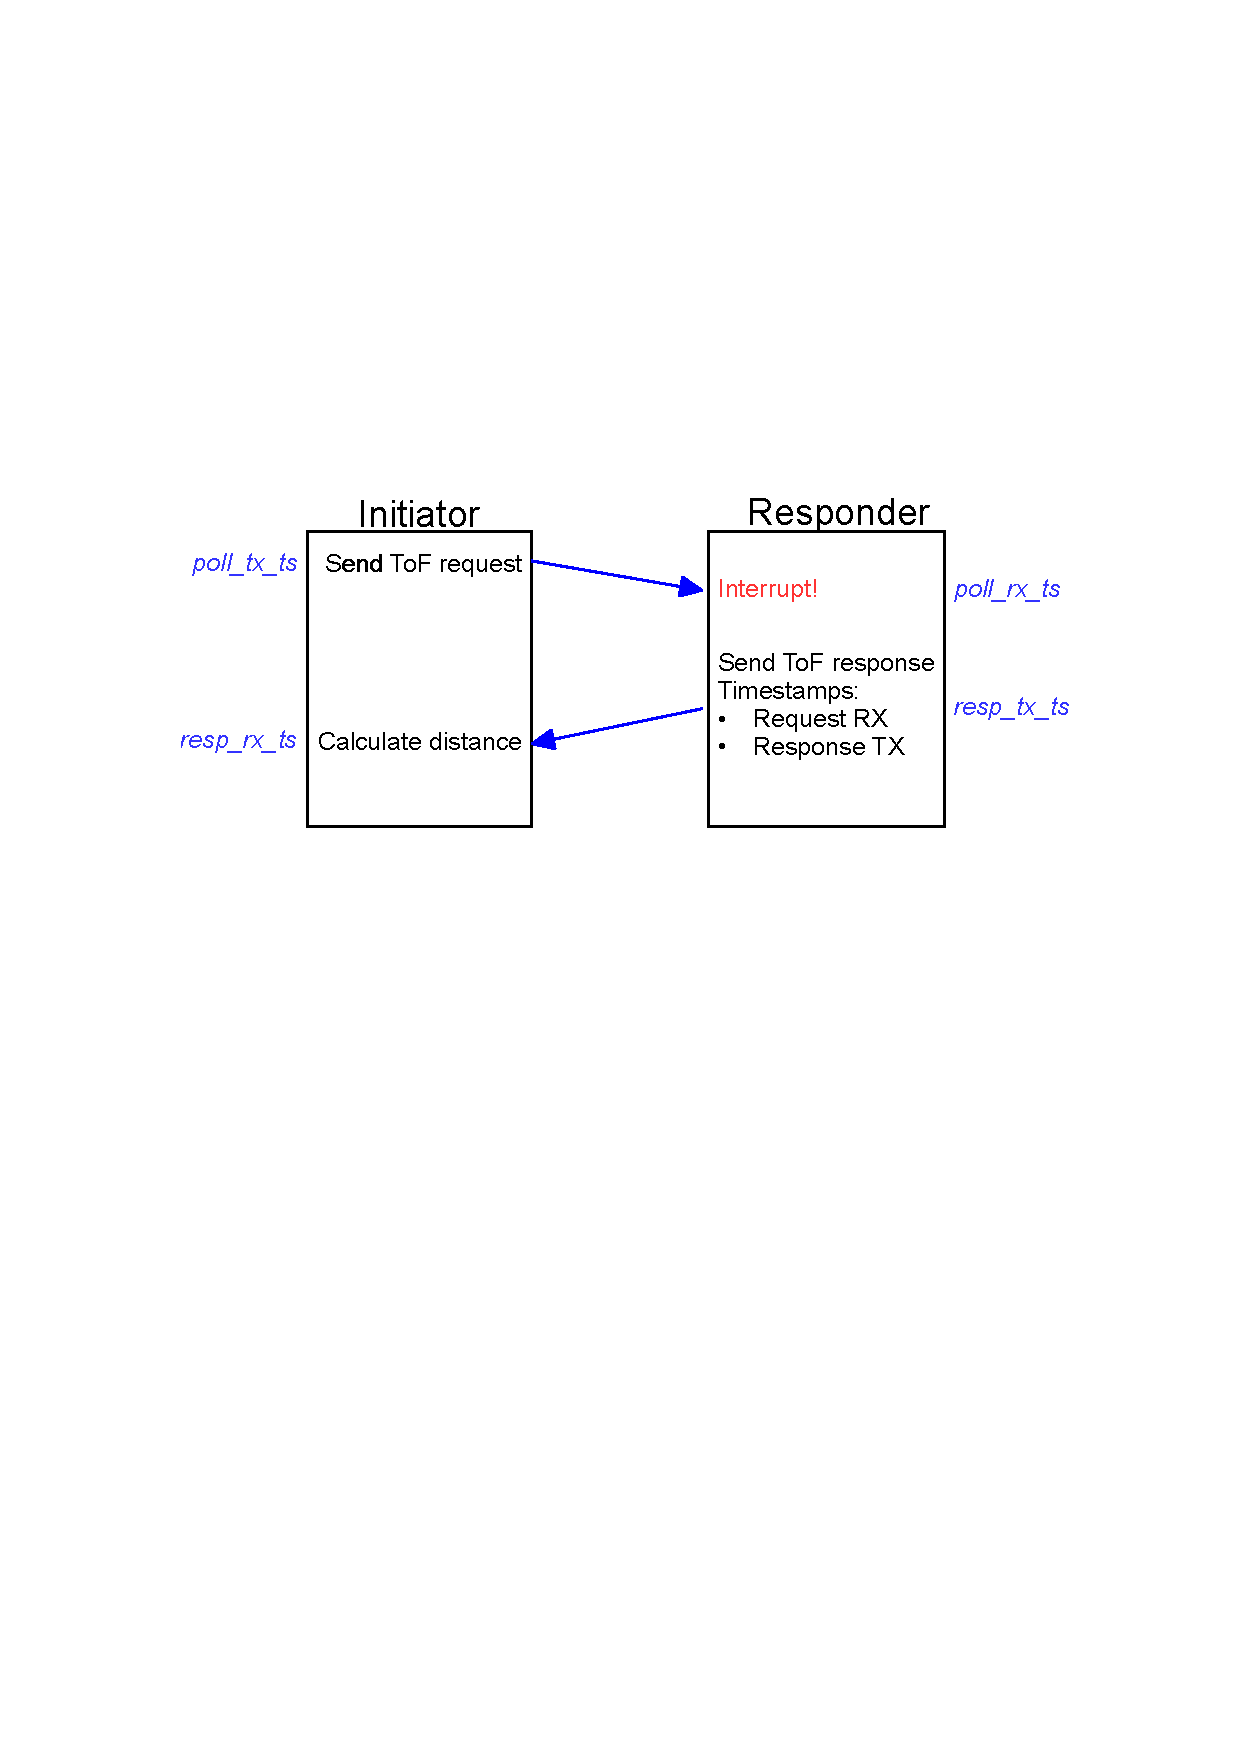
\includegraphics[width=0.8\textwidth]{pictures/ToF_scheme.pdf}
		\caption{Sketch of the complete setup.}
		\label{fig:tof_sketch}
	\end{figure}
\end{center}


To estimate the distance, four timestamps, marked in blue in Figure \ref{fig:tof_sketch}, are used. These timestamps are expressed in ticks and are stored in a 32-bit variable. The timestamps are as follows:

\begin{center}
	\begin{table}[!hbt]
		\begin{tabular}{ | m{5em} | m{10cm} |} 
			\hline
			poll\_tx\_ts & Time of request being sent by Initiator \\ 
			\hline
			poll\_rx\_ts & Time of request being received by Responder \\ 
			\hline
			resp\_tx\_ts & Time of response being sent by Responder \\ 
			\hline
			resp\_rx\_ts & Time of response being received by Initiator \\ 
			\hline
		\end{tabular}
		\caption{Timestamp variables.}
		\label{tab:timestamps}
	\end{table}
\end{center}

To calculate the time it took for the poll message to travel from the initiator to the responder, the \blueconsolas{poll\_tx\_ts} timestamp is subtracted from the \blueconsolas{poll\_rx\_ts} timestamp, yielding the \blueconsolas{rtd\_init} value. Similarly, for the time the response message took to travel in the opposite direction, \blueconsolas{resp\_tx\_ts} is subtracted from \blueconsolas{resp\_rx\_ts}, resulting in the \blueconsolas{rtd\_resp} variable.
\vspace{4pt}
\newline
To determine the distance between the initiator and the responder, the two times (\blueconsolas{rtd\_init} and \blueconsolas{rtd\_resp}) are averaged. Before averaging, the response time (\blueconsolas{rtd\_resp}) is adjusted by applying an offset factor (1 - clockOffsetRatio). This compensates for potential variations that may arise if the clock of the initiator runs slightly faster or slower than the responder due to factors such as aging effects, temperature, voltage, or manufacturing discrepancies.
\vspace{4pt}
\newline
Finally, to compute the distance between the two devices, the average time is converted to seconds and then multiplied by the predefined speed of light, representing the speed of electromagnetic field expansion.
\vspace{4pt}
\newline
This process is subsequently repeated for all of the saved anchors to get the distance to every single one. 
The calculated distances are saved in the distances array. 



\section{TofDevice}
\label{sec:TofDevice}
The TofDevice class is a base class for Tof devices, serving as a superclass for both TOF initiators and responders. 
It encapsulates common functionality and configurations required for TOF devices using the DW3000 chip.
The class provides methods for initializing and configuring the TOF device, starting a watchdog timer for handling failure events, enabling LEDs for debugging, and implementing the main loop for the TOF device.
Additionally, it includes parameters and configurations specific to the DW3000 chip, such as communication settings, encryption keys, and antenna delay values.

\subsection{TofDevice Variables}
\label{subsec:TofDevice_Variables}

\subsubsection{Constants}
\begin{itemize}
	\item \textbf{DEST\_PAN\_ID}
	\newline
	desc
	\item \textbf{START\_RECEIVE\_DATA\_LOCATION}
	\newline
	desc
	\item \textbf{ALL\_MSG\_SN\_IDX}
	\newline
	desc
	\item \textbf{RESP\_MSG\_POLL\_RX\_TS\_IDX}
	\newline
	desc
	\item \textbf{RESP\_MSG\_RESP\_TX\_TS\_IDX}
	\newline
	desc
	\item \textbf{RESP\_MSG\_TS\_LEN}
	\newline
	desc
	\item \textbf{INITIATOR\_KEY\_INDEX}
	\newline
	desc
	\item \textbf{RESPONDER\_KEY\_INDEX}
	\newline
	desc
	\item \textbf{RX\_BUF\_LEN}
	\newline
	desc
	\item \textbf{TX\_ANT\_DLY}
	\newline
	desc
	\item \textbf{RX\_ANT\_DLY}
	\newline
	desc
\end{itemize}

\subsubsection{Private Variables}
\begin{itemize}
	\item \textbf{Watchdog my\_watchdog}
	\newline
	The my\_watchdog variable is an instance of the Watchdog class, representing a software watchdog timer used to monitor the proper execution of the TOF device's main loop. It is initialized with a timeout value, and its purpose is to reset the device if the timer is not reset within the specified duration, enhancing the device's reliability and fault tolerance. The section\ref{sec:Watchdog_Handling} delves into the watchdog class.
	
	\item \textbf{uwb\_addr src\_address}
	\newline
	The src\_address of type long long holds a 32-Bit UWB address. 
	
	\item \textbf{String type}
	\newline
	The type variable of type String holds the information whether the device is identified as tag or responder. 
	
	\item \textbf{mac\_frame\_802\_15\_4\_format\_t mac\_frame}
	\newline
	The mac\_frame variable is of the type mac\_frame\_802\_15\_4\_format\_t and used to construct and alter the UWB message corresponding to the IEEE 802.15.4 communication standard. 
	
	\item \textbf{uint8\_t poll\_msg[4]}
	\newline
	poll\_msg is a four byte array representing the specific poll message payload. 
	In this case it is labeled {'P', 'o', 'l', 'l'} and is used by the tag ot initiate a UWB cycle. 
	
	\item \textbf{uint8\_t resp\_msg[16]}
	\newline
	The resp\_msg is similar to the poll\_msg used to construct MAC frames. 
	In this case the message is 16 bytes ling with the first 8 bytes reserved for the timestamps of the responder. The last 8 bytes carry the characters 'R', 'e', 's', 'p', 'o', 'n', 's', 'e' indicating the nature of the message. 
	
	\item \textbf{uint8\_t rx\_buffer[RX\_BUF\_LEN]}
	\newline
	The rx\_buffer array allocates memory to store a incoming UWB message of the maximum size. 
	
	\item \textbf{uint32\_t status\_reg}
	\newline
	The status\_reg holds information about the process of a message being sent. 
	It masks errors and timeouts that may occur when a UWB message is transmitted or received. 
	
	\item \textbf{dwt\_aes\_job\_t aes\_job\_tx, aes\_job\_rx}
	\newline
	Both aes\_job\_tx and aes\_job\_rx are of the struct type dwt\_aes\_job\_t and contain information needed for the AES encryption/decryption of each MAC frame being send or received. 
	
	\item \textbf{int8\_t status}
	\newline
	The status variable is used to save and evaluate the status of a AES encryption. It masks different AES errors to its bits. 
	
	\item \textbf{dwt\_aes\_config\_t aes\_config}
	\newline
	The aes\_config variable represents an instance of the dwt\_aes\_config\_t type. 
	It is used to configure and specify parameters for the AES operations within the TOF device. 
	The dwt\_aes\_config\_t type includes fields for selecting the AES core type, setting the key source, and defining other encryption-related configurations. 
	
	\item \textbf{dwt\_config\_t config}
	\newline
	The config variable is an instance of the dwt\_config\_t type, and it is used to store configuration parameters related to the DW3000 chip, which is used for TOF communication. 
	The dwt\_config\_t type includes fields such as channel number, preamble length, data rate, and other settings that determine the behavior of the DW3000 chip during communication. 
	This variable is utilized in the setup process to initialize and configure the TOF device for proper operation.
	
	\item \textbf{dwt\_aes\_key\_t keys\_options[NUM\_OF\_KEY\_OPTIONS]}
	\newline
	The keys\_options variable in the TofDevice class is an array of dwt\_aes\_key\_t elements. 
	It is used to store different encryption keys for AES operations within the TOF device. 
	Each element in the array (dwt\_aes\_key\_t) represents a set of encryption keys, allowing for multiple key options. 
	These keys are used to secure communication between TOF devices, providing a level of cryptographic protection for the transmitted data.
\end{itemize}

\subsection{TofDevice Constructor}
\label{subsec:TofDevice_Constructor}
The TofDevice constructor initializes a new instance of the TofDevice class within the Device namespace. It takes two parameters: uwb\_addr src for the source address of the TOF device and unsigned long wdt\_timeout for the watchdog timer's timeout duration. 
It begins by initializing SPI comminication to the DWM3000 chip and ensuring that it is in a stable state after startup through a soft reset and a brief delay. 
Subsequently, it checks the device's idleness in the Idle RC state before proceeding. 
The method then initializes the DW3000 chip using the dwt\_initialise function. 
If any of these steps fail, it prints error messages and enter a loop indicating failure. 
Lastly the config data for the operation of the DWM and the AES encryption as well as are the keys\_options set in the corresponding variables config, aes\_config and keys\_options are set

\subsection{virtual void setup}
\label{subsec:TofDevice_setup}
The setup method in the TofDevice class serves as the initialization routine for the TOF device. 
It uses the dwt\_configure function to configure the DWM3000 with the config options set in the constructor describes in \ref{subsec:TofDevice_Constructor}. 
If this fails it will print an error message and go in a loop. 
The configuration of the transmission spectrum parameters is handled by dwt\_configuretxrf, and default antenna delay values are applied through dwt\_setrxantennadelay and dwt\_settxantennadelay. 

\subsection{void start\_wdt}
\label{subsec:TofDevice_start_wdt}
The start\_wdt method in the TofDevice class initiates the watchdog timer associated with the TOF device using the begin method of the Watchdog class targeted in \ref{subsec:Watchdog_begin}. This method is responsible for commencing the timer, which monitors the execution of the device's main loop. 

\subsection{void enable\_leds}
\label{subsec:TofDevice_enable_leds}
The enable\_leds method activates the RX and TX LEDs for debugging purposes. 
By enabling the LEDs, each transmission triggers a visual indication of sent and received messages, aiding in the debugging process. Note that in practical low-power applications, LEDs might be disabled to conserve power, but in a debug scenario or when the device is hooked up to a stable supply like the main grid. 

\subsection{virtual void loop}
\label{subsec:TofDevice_loop}
The loop method represents the main operational loop for the TOF device. 
Within this loop, the device continually resets the watchdog timer using the resetTimer method, ensuring that the device remains within its expected operational timeframe. 

\subsection{char* get\_type}
\label{subsec:TofDevice_get_type}
The private get\_type method returns a pointer to the type variable of the TOF device seen in \ref{subsec:TofDevice_Variables}, offering a descriptive label for the TOF device's classification.

\section{TofInitiator}
\label{sec:TofInitiator}
The TofInitiator class is a subclass of TofDevice and represents a TOF initiator device. 
It extends the base class functionality to handle TOF request transmissions, response processing, and secure communication with responder devices. 
The class encapsulates frame construction, nonce generation, and specific logic for managing communication with multiple responders.

\subsection{TofInitiator Variables}
\label{subsec:TofInitiator_Variables}

\subsubsection{Extern Variables}
\begin{itemize}
	\item \textbf{extern double distances[NUM\_LANDMARKS]}
	\newline
	The distances variable is an external array declared as extern double 
	\newline
	distances[NUM\_LANDMARKS] in the tof-initiator.h file. 
	This array is initialized in ther main.cpp file and is intended to store distance measurements calculated by the TOF initiator for each responder in the system. 
	The size of the array, NUM\_LANDMARKS, is determined by the number of responders in the system, and each element in the array holds the calculated distance for a specific responder. 
	The actual values are be updated during the processing of TOF responses in the process\_tof\_response method as described in \ref{subsec:TofInitiator_process_tof_response}.
\end{itemize}

\subsubsection{Private Variables}
\begin{itemize}
	\item \textbf{uint32\_t frame\_cnt}
	\newline
	The frame\_cnt variable represents the frame count, tracking the number of frames transmitted by the TOF initiator. 
	It is incremented after each transmission and is used to manage frame sequencing within the communication protocol. 
	This count helps maintain synchronization and order in the communication between the initiator and responder devices.
	
	\item \textbf{seq\_cnt}
	\newline
	The seq\_cnt variable represents the frame sequence number, and it is used to keep track of the sequence of frames transmitted by the TOF initiator. 
	It is incremented after each transmission to ensure that each frame has a unique identifier within the communication protocol. 
	The seq\_cnt value is part of the frame's metadata and aids in maintaining order and synchronization between the initiator and responder devices in the TOF communication system.
	
	\item \textbf{uint8\_t nonce[13]}
	\newline
	The nonce variable is a 13-byte array used as a nonce (Number used Once) in the context of secure communication. 
	It serves as a unique value for each frame transmission and is utilized in the encryption and decryption processes to enhance security by preventing replay attacks. 
	The nonce is generated and updated for each TOF frame transmission, contributing to the integrity of the communication between the TOF initiator and responder devices.
	
	\item \textbf{dst\_address}
	\newline
	The dst\_address variable is a pointer to an array of destination addresses for the responders. 
	It represents the target addresses to which the TOF initiator sends its requests. 
	The array holds the addresses of all individual responder devices, and the TofInitiator class uses this information to selectively communicate with each responder one after another during the TOF communication process.
	
	\item \textbf{uint8\_t total\_responders}
	\newline
	The total\_responders variable represents the total number of responder devices that the TOF initiator communicates with. 
	It indicates the size of the array of destination addresses (dst\_address) and helps manage the looping through responder devices during the TOF communication process. 
	The TOF initiator iterates through the responders, sending TOF requests and processing responses, and total\_responders determines the number of devices in this communication setup.
	
	\item \textbf{uint8\_t current\_responder}
	\newline
	The current\_responder variable is an index used to keep track of the current responder being communicated with during the TOF communication process. 
	It is incremented and looped to iterate through the array of destination addresses (dst\_address), allowing the TOF initiator to selectively send TOF requests and process responses from different responder devices. 
	This index management facilitates sequential communication with multiple responders within the specified array.
	
	\item \textbf{double tof}
	\newline
	The tof variable represents the calculated Time-of-Flight for a particular communication instance. 
	It is used to store the calculated time it takes for a signal to travel from the TOF initiator to the responder and back. 
	The tof value is derived during the processing of TOF responses and is an essential parameter for determining the distance between devices using the speed of light.
	
	\item \textbf{double temp\_distance}
	\newline
	The temp\_distance variable is used to buffer the calculated distance based on the Time-of-Flight measurement during the processing of TOF responses. 
	It represents a temporary variable for storing the distance information before it may be further utilized in the application. 
\end{itemize}

\subsection{TofInitiator Constructor/Dectructor}
\label{subsec:TofInitiator_Constructor}
The TofInitiator constructor takes parameters representing the source address for the TOF initiator (src), an array of destination addresses for the responders (dst), the watchdog timer timeout value (wdt\_timeout), and the number of responder devices (num\_of\_responders). 
It sets the type String variable to "Initiator" indicating its role, initializes tof, temp\_distance and frame\_cnt with 0 and seq\_cnt to 10 (0x0A). 
Latly the MAC-Frame is assembled. 

\subsection{virtual void setup}
\label{subsec:TofInitiator_setup}
The setup method initializes the TOF initiator by calling the base class's setup method to configure basic parameters descibed in \ref{subsec:TofDevice_setup}. 
It then sets the expected response delay and timeout using the dwt\_setrxaftertxdelay and dwt\_setrxtimeout functions. 
After that the parameters for the AES are set for rx encryption and tx decryption. 

\subsection{virtual void loop}
\label{subsec:TofInitiator_loop}
The loop method serves as the central processing hub, orchestrating the continuous operation of the TOF initiator device. 
It begins by invoking the base class loop method, decribed in \ref{subsec:TofDevice_loop}, which includes resetting the watchdog timer to prevent system resets due to potential failures. 
\vspace{4pt}
\newline
Within the loop, the current\_responder index is iteratively updated, allowing the TOF initiator to cycle through the array of destination addresses. 
For each iteration, a TOF request is sent to the selected responder using the send\_tof\_request function. 
After sending the method checks certain bits in the status\_reg variable to ensure the message was being sent correctly and if so, updates the seq\_cnt and frame\_cnt counters. 
\vspace{4pt}
\newline
The method then enters a loop until it detects a response message being received by checking the SYS\_STATUS\_RXFCG\_BIT\_MASK masked in the status\_reg variable. 
Then the method processes the response by calling the process\_tof\_response described in \ref{subsec:TofInitiator_process_tof_response} and puts it in the distances array. 

\subsection{void send\_tof\_request}
\label{subsec:TofInitiator_send_tof_request}
The send\_tof\_request method is responsible for initiating and sending a TOF request to a specific destination address (responder) and is called in the loop function \ref{subsec:TofInitiator_loop}. 
It method sets the correction key, assembles the MAC frame and configures and initiates the AES encryption. 
If the encryption is unsuccessful, a error message will be printed on the serial monitor and the method ends. 
Otherwise the frame is assembled and the transmission is stated using the dwt\_starttx function. 
By setting the two masked bits DWT\_START\_TX\_IMMEDIATE and DWT\_RESPONSE\_EXPECTED the message is sent without a delay and the initiator is set to wait for a response.  

\subsection{void process\_tof\_response}
\label{subsec:TofInitiator_process_tof_response}
The process\_tof\_response method is responsible for handling and extracting relevant information from a TOF response received from a responder device. 
It method begins by clearing the indication of a good received frame in the status register. It then reads the length of the received frame and proceeds to decrypt the payload of the response using AES decryption after putting it in the rx\_buffer variable. 
The method checks for potential errors in the decryption process and throws error messages over the serial monitor if so. 
\vspace{4pt}
\newline
Upon successful decryption, the method verifies that the received frame matches the expected response from the TOF responder. It extracts the relevant timestamps from the response payload, computes the Time-of-Flight (TOF) and distance based on these timestamps, and updates the tof and temp\_distance variables like discussed in the Distance Measurement section \ref{sec:Distance_Measurement}. 

\section{TofResponder}
\label{sec:TofResponder}
The TofResponder class extends the TofDevice class and is responsible for configuring and operating as a TOF responder device. 
It includes methods for setup and continuous operation in the main loop. 
The class utilizes AES encryption for secure communication and employs interrupts to handle successful frame reception. 
Additionally, it maintains a FreeRTOS Semaphore (responseSemaphore) to coordinate the response process, and it updates RX diagnostics information during operation.

\subsection{TofResponder Variables}
\label{subsec:TofResponder_Variables}
\subsubsection{Private Variables}
\begin{itemize}
	\item \textbf{uwb\_addr dst\_address}
	\newline
	The 32-bit dst\_address variable of type long long holds the destination address to which the responder sends its response. This address is set during the instantiation of a TofResponder object and is used to ensure that the response is sent to the initiator device.
	
	\item \textbf{uint64\_t poll\_rx\_ts}
	\newline
	The poll\_rx\_ts variable holds the timestamp when the TOF responder receives a poll frame from the TOF initiator. This timestamp is essential for calculating the time of flight and is put in the response frame. 
	
	\item \textbf{uint64\_t resp\_tx\_ts}
	\newline
	The resp\_tx\_ts variable holds the timestamp when the TOF responder transmits the response frame to the TOF initiator. 
	This timestamp is used in conjunction with the poll\_rx\_ts to calculate the time-of-flight and derive accurate distance measurements in the initiator. 
	Therefore it is also sent back in the response frame
	
	\item \textbf{DynamicJsonDocument* rx\_diagnostics\_json}
	\newline
	The rx\_diagnostics\_json is a pointer to a DynamicJsonDocument object. 
	This object is used to store diagnostic information, such as timing and status parameters, related to the reception of frames by the TOF responder. 
	The use of a JSON document allows for flexible and structured storage of diagnostic data, facilitating analysis and debugging.
	
	\item \textbf{static SemaphoreHandle\_t responseSemaphore}
	\newline
	The responseSemaphore is a static semaphore in the TofResponder class, implemented using FreeRTOS. 
	It serves as a mechanism to control the flow of the program, specifically signaling the main loop when it's time to send a response. 
	The semaphore is initially unavailable, and it is given (made available) from within the ISR (rx\_ok\_cb) when a valid frame is received, allowing the main loop to proceed with handling the response.
	
\end{itemize}

\subsection{TofResponder Constructor/Dectructor}
\label{subsec:TofResponder_Constructor}
The TofResponder constructor takes four parameters: uwb\_addr src (source address of the specific responder), uwb\_addr dst (destination address of the initiator), unsigned long wdt\_timeout (watchdog timeout in milliseconds), and DynamicJsonDocument* rx\_diagnostics (pointer to a JSON document for receive diagnostics), setting it up with the rx\_diagnostics\_json member variable. 
\vspace{4pt}
\newline
The constructor sets the type member variable to "Responder", creates a static semaphore (responseSemaphore) for synchronization and initializes it as unavailable. 
If the semaphore creation fails an error message is printed on the serial monitor. 

\subsection{virtual void setup}
\label{subsec:TofResponder_setup}
The setup method first calls the TofDevice::setup() method described in \ref{subsec:TofDevice_setup} to perform general setup tasks. 
Then, it configures the Transmit (TX) and Receive (RX) Advanced Encryption Standard (AES) jobs for encryption and decryption tasks, respectively. 
Subsequently it sets the rx\_ok\_cb method described in \ref{subsec:TofResponder_rx_ok_cb} as a callback function for a UWB message being received using the dwt\_setcallbacks function and then configures the DWM3000 to throw an interrupt whenever a good frame is received using the dwt\_setinterrupt and port\_set\_dwic\_isr functions. 
Lastly the method configures additional diagnostics using the dwt\_configciadiag allowing channel state informations being extracted after each received frame. 

\subsection{virtual void loop}
\label{subsec:TofResponder_loop}
The loop method is the main operational loop for the TOF responder device. 
It begins by invoking the TofDevice::loop() method to reset the watchdog timer. 
Subsequently, it activates reception immediately using dwt\_rxenable(DWT\_START\_RX\_IMMEDIATE). 
The method then waits for a semaphore signal (responseSemaphore) to indicate an active response, and upon receiving the signal, it proceeds to process the received frame as follows.
\vspace{4pt}
\newline
Within the response processing section, the method checks if the received frame matches the expected poll from the TOF initiator. 
If the message can not be decypted correctly, for example when the poll message is destined at another responder device, an error message is thrown on the serial monitor and the function returns immediately. 
\vspace{4pt}
\newline
If the check passes, the message is put in the rx\_buffer and a response message is assembled by getting the timestamp when the poll was received (poll\_rx\_ts) and calculating a time when the response is estimated to be sent (resp\_tx\_ts). 
This requires the POLL\_RX\_TO\_RESP\_TX\_DLY\_UUS parameter to be well tuned like explained in chapter \ref{chap:Tuneable Parameters} as well as the antenna delay also being added. 
\vspace{4pt}
\newline
Then the message is assembled by putting the two times poll\_rx\_ts and resp\_tx\_ts and generating the MAC frame. 
With that being done the AES is configured and the message is encrypted. 
When encrypting is done the UWB message is sent using the dwt\_starttx function and its return value is examined if any errors occurred. 
If so, the device will enter a loop, otherwise the corresponding registers are cleared and the update\_rx\_diagnostics (referenced in \ref{subsec:TofResponder_update_rx_diagnostics}) function is called. 

\subsection{void update\_rx\_diagnostics}
\label{subsec:TofResponder_update_rx_diagnostics}
The update\_rx\_diagnostics method is responsible for updating the receiver diagnostics information. 
It extracts relevant diagnostic data from the DWM3000 module and updates a JSON document (rx\_diagnostics\_json) with this information. 
The diagnostic data includes parameters such as reception times, status, phase of arrival, power levels, frequency-related information, and other accumulated counts.
\vspace{4pt}
\newline
The method employs the dwt\_readdiagnostics function to retrieve the relevant diagnostic data. 
It then populates the corresponding fields in the JSON document with the retrieved values. 
This updated diagnostic information can be utilized for monitoring and analysis of the TOF responder's receiver performance. 

\subsection{static void rx\_ok\_cb}
\label{subsec:TofResponder_rx_ok_cb}
The rx\_ok\_cb method is a static interrupt service routine (ISR) for handling the event of a successful frame reception. 
This callback is registered with the DW3000 IC and is invoked when a good frame is received. 
Its primary purpose is to release a FreeRTOS semaphore (responseSemaphore) to indicate that an active response is available for further processing in the main loop.
\vspace{4pt}
\newline
Upon receiving a good frame, the method calls xSemaphoreGiveFromISR to release the semaphore. This allows the main loop, which is potentially waiting for a response, to proceed with processing the received frame. Additionally, the method checks whether a higher-priority task needs to be woken up, and if so, it requests a context switch using portYIELD\_FROM\_ISR.

\section{Watchdog Handling}
\label{sec:Watchdog_Handling}
To ensure that the UWB task on all devices keeps being up and running to deliver data for continuing to estimate the tag's position and is not interrupted or halted in an infinite loop a watchdog logic is implied in the TofDevice class. 
The watchdog is implemented in the "watchdog.h" and "watchdog.cpp" files. 
The timer used is given by FreeRTOS xTimer functionality. 

\subsection{Watchdog Variables}
\label{subsec:Watchdog_Variables}

\subsubsection{private Variables}
\begin{itemize}
	\item \textbf{unsigned long timeoutMillis}
	\newline
	Holds the duration in milliseconds after the watchdog will fire. 
	\item \textbf{TimerHandle\_t timer}
	\newline
	Holds FreeRTOS timer handle of type TimerHandle\_t. 
\end{itemize}

\subsection{Watchdog Constructor}
\label{subsec:Watchdog_Constructor}
When constructing a Watchdog object the constructor takes in the timeoutMillis variable of type unsigned long and assigns it. 

\subsection{void resetTimer}
\label{subsec:Watchdog_resetTimer}
The resetTimer Method takes in no parameters and resets the timer object of type TimerHandle\_t to 0 using the FreeRTOS xTimerReset function. 

\subsection{void begin}
\label{subsec:Watchdog_begin}
The begin Method creates the timer of type TimerHandle\_t using the FreeRTOS xTimerCreate fuction. 
It assigns the name "WatchdogTimer", the timeout period and the timerCallback method as a callback dunction that is fired once the designated time is elapsed. 
Then it is checked if the timer creation was successful and the timer is started using FreeRTOS function xTimerStart. 
If the timer creation as unsuccessful an error message will be outputted via UART. 

\subsection{void stop}
\label{subsec:Watchdog_stop}
The stop method checks if a timer object is present. 
If so it is stopped and deleted by the FreeRTOS functions xTimerStop and xTimerDelete. 

\subsection{unsigned long get\_timeout}
\label{subsec:Watchdog_get_timeout}
The get\_timeout method, when called, acts as a getter function and returns the current timeout period saved in the timeoutMillis variable of type unsigned long. 

\subsection{static void timerCallback}
\label{subsec:Watchdog_timerCallback}
The timerCallback function is called every time duration in timeoutMillis is elapsed. 
When called the function prints a serial message that the watchdog timer has elapsed and then restarts the esp device using the esp\_restart function. 
